% \textcolor{red}{[additional motivation for coala memory virtualization] we should emphasize that Coala programming model removes the burden of identifying the write-after-read dependencies from the programmer  as compared to Chain. And it does not require a specific compiler that cannot consider a runtime dependent behavior like Interrupts service handling to guarantee memory protection, as in Alpaca.}
%
\sys's {\em virtual memory manager} (VMM) abstracts the physical address space of the non-volatile memory (FRAM) and divides it into \texttt{\underline{private}} and \texttt{\underline{shadow}} (underlined locations are non-volatile) buffers. Each buffer is divided into pages. The VMM prohibits applications from directly access these buffers. Instead, it redirects any request to the \texttt{working} buffer located in the volatile memory (SRAM), which has a lower latency and energy cost to access than FRAM. It populates \texttt{working} buffer with the privatized pages from non-volatile memory. When a coalesced task completes, the VMM ensures that updated pages are committed to main memory and visible to subsequently executed tasks. If the power interrupts a task, the VMM ensures the consistency of the data by relying on its \texttt{\underline{private}} buffer. The VMM ensures consistency even if a task or a sequence of tasks include WAR dependences that could compromise consistency~\cite{ratchet,dino}.
%
On a commit, the VMM atomically copies all ``dirty'' pages back into their location in the non-volatile memory.
%
SRAM has a limited size and there is an extended working memory containing {\em
shadow pages} in the larger FRAM.  A shadow page stores the data from an
updated pages that need to be committed back to non-volatile memory, but that
exceeded the size of the volatile working memory.
%
the VMM moves pages of data efficiently using hardware accelerated Direct Memory
Access (DMA) support, which copies a block of memory from one place to another
as a single operation.\\
%
\begin{figure}
    \centering
    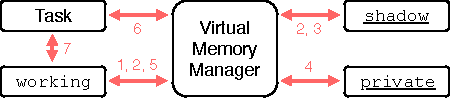
\includegraphics[width=\columnwidth]{figures/mem-man.pdf}
    \caption{Interaction between task, memory manager and memory buffers upon \texttt{RP} and \texttt{WP},
    and order of occurrence. Steps 2, 3, 4 and 5 are conditional. Tasks only have direct access to the
    \texttt{working} buffer.}
    \label{figure:mem-man}
\end{figure}
%
\textbf{System Overview.}
Figure~\ref{figure:mem-man} gives an overview of \sys's virtual memory management system,
whose details are provided throughout this section.
A page has a home location in non-volatile memory which we refer to as the page's
\texttt{\underline{private}} (underlined locations are non-volatile).  When a
task accesses a page, the VMM swaps the page from its home location
into the fully\hyp{}associative \texttt{working} buffer that is stored in
volatile memory.  The \texttt{working} buffer is allocated to take up the
volatile memory that remains after space for stack is allocated.
%
The VMM utilizes a two-phase commit to write dirty pages from the \texttt{working}
buffer back to their home location in \texttt{\underline{private}}. It optimizes this process by using an indirection table to abstract the location of the \texttt{\underline{private}} buffer and
to eliminate the need for the second page copy.
%
The VMM is forced to swap out a dirty page from the \texttt{working} buffer
when a task requests a page that is not in the \texttt{working} buffer, and there is no
free page in the working buffer (i.e., a page fault). On a page fault, the VMM
moves the page to the direct\hyp{}mapped non-volatile \texttt{\underline{shadow}} buffer. \\
%
\subsection{Address Translation and Variable Access}
%
A task must access protected non-volatile variables through \sys's
restricted memory interface. The interface includes \texttt{RP}$(v)$, to read the value of variable
$v$, and \texttt{WP}$(v)$ to assign a value to variable $v$. The
implementation of {\tt RP} is shown in Algorithm~\ref{algo:rwar}, and {\tt
WP}'s implementation is similar except that {\tt WP} marks the accessed page as
dirty.
%
{\tt RP} and {\tt WP} operations translate a variable's physical address in
non-volatile memory into a \emph{virtual address} in \texttt{working} buffer in
volatile memory. In \sys, a virtual address is composed of a \emph{page tag}
that identifies the page and a \emph{page offset} that identifies a byte.
%
\begin{figure}
\fbox{\parbox{\linewidth}{
	\captionof{algorithm}{\texttt{RP}(variable $v$)}
	\label{algo:rwar}
	\scriptsize
	\begin{algorithmic}[1]
		\State $t \leftarrow \Call{GetTag}{v}$
        \State $i \gets \{ j\ |\ \Call{GetTag}{\texttt{working}[j]} = t \}$ \Comment{Search page}
		\If { $i = \emptyset$ } \Comment{Var in a resident page?}
		\State	$i \gets \Call{PageFault}{t}$ \Comment{Swap page in}
		\EndIf
		\State $o \leftarrow \Call{GetOffset}{v}$
		\State \Return \texttt{working}[$i$][$o$]  \Comment{Return from page}
	\end{algorithmic}}}
\end{figure}
%
After address translation (Figure~\ref{figure:mem-man}, Step 6), a task
accesses the protected variable's location in the volatile \texttt{working} buffer
(Step 7). \sys keeps track of the page tags for
the pages currently resident in the \texttt{working} buffer. When a task accesses a
variable, it compares the variable's page tag to tags of the pages in {\tt
working} (Algorithm~\ref{algo:rwar}, Line 2).
%
If the accessed variable's page tag is not found in the page buffer, the
operation incurs a {\em page fault} (Line 4).
%
The byte is accessed in the page buffer at the index of the resident page and
the variable's page offset (Lines 5--6).
%
\subsection{Page Faults and Page Swapping}
%
When accessing a protected variable with \texttt{RP} or \texttt{WP}, the memory
manager first searched the variable's page in the \texttt{working} buffer
(Figure~\ref{figure:mem-man}, Step 1).
If the page is not found there, a page fault is incurred and a new page needs to
be swapped in.
If the \texttt{working} buffer is full, a page fault on a memory access
requires VMM to swap out one of the pages in the \texttt{working} buffer (a
\emph{victim page}) preserving updates made to that page.
%
While we opted for the simplicity of FIFO, any other replacement policy, such
as Least Recently Used (LRU) could work in its place. \\
%
If a task modified any byte in the victim page (i.e., using \texttt{WP}), then
the page is dirty and its changes has to be persisted to non-volatile memory
(Figure~\ref{figure:mem-man}, Step 2).
If the accessed page was previously modified and swapped out since the last
power failure, the most recent version of the page is in {\tt
\underline{shadow}} (Step 3), otherwise it has to be retrieved from
{\tt \underline{store}} (Step 4).
Finally, the page is copied to the volatile buffer (Step 5). \\
%
\subsection{Atomic Two-Phase Commit of Dirty Pages}
%
When the last task in a sequence of coalesced tasks completes, \sys must commit
\emph{all} dirty pages in the \texttt{working} buffer and in the
\texttt{\underline{shadow}} buffer, copying them back to their original
locations in the main memory \texttt{\underline{private}}. If a task were allowed
to (re-)execute after only some pages have been committed to
\texttt{\underline{store}}, the task might see protected variables in an
inconsistent state; \sys's two-phase commit prevents this inconsistency. \\
%
To make the commit atomic, \sys commits the pages in two phases, implemented by
Algorithm~\ref{algo:commit}.
%
The first phase copies dirty pages from the \texttt{working} buffer to the
non-volatile \texttt{\underline{shadow}} buffer (Line 4). The second phase
commits pages from \texttt{\underline{shadow}} to \texttt{\underline{store}}
(Line 12).  If power fails during the first phase, the whole commit is aborted,
and the execution restarts from the most recently committed point (i.e., from
the first task in a coalesced sequence of tasks). If power fails in the second
phase, the commit process safely resumes on reboot.  The second phase of commit
depends on some run-time metadata. The \texttt{\underline{committing}} bit
indicates that a commit is in progress and is set before the first page is
committed (Line 9) and cleared after the last page is committed (Line 16).  The
\texttt{\underline{shadowCount}} records the number of dirty shadow pages to
commit and \sys clears the counter when commit completes (Line 14).  The
\texttt{\underline{commitIndex}} indexes the next page to be committed (Line
11) and \sys clears the index at the end of the phase (Line 15).
%
\sys's commit is efficient because it maintains an index dirty pages instead of
iterating through all potentially dirty pages to check a dirty bit during
commit.
%
\sys's implementation is also efficient because the memory manager does not
copy from \texttt{\underline{shadow}} to \texttt{\underline{store}}, instead
swapping pointers in an indirection table that maintains the pages as a double
buffer.  Section~\ref{sec:implementation} describes double buffering in more
detail. \\
%
\textbf{Memory Consistency.} \sys's paging mechanism ensures that a task only
ever executes using consistent protected data. During task execution,
modifications to protected data do not affect their original memory locations,
because a task reads and writes the volatile \texttt{working} buffer only, and
modified pages are kept in \texttt{\underline{shadow}} until commit.  A power
failure erases the contents of the page buffer, preventing a re-executing task
from observing updates in the page buffer from a previous execution attempt.
Clearing \texttt{\underline{shadowCount}} as part of the second phase commit
(Line 14), ensures that all accesses to protected variables in subsequent tasks
correctly access their original memory locations in \texttt{\underline{store}}.
\sys assumes that the write to a non-volatile word in memory is atomic. \\
%
\begin{algorithm}[t]
	\caption{Two-phase commit}
	\label{algo:commit}
	\scriptsize
	\begin{algorithmic}[1]
        \Procedure{CommitPhase1}{} \Comment{On last coalesced task}
            \For {$i \in 0..|\texttt{working}|-1$}
                \State $t \gets \Call{Tag}{\texttt{working}[i]}$
                \State $\texttt{\underline{shadow}}[\Call{Tag}{\texttt{working}[i]}] \xleftarrow{\text{DMA}} \texttt{working}[i]$
                \State $\texttt{\underline{shadowList}}[\texttt{\underline{shadowCount}}] \gets t$
                \State $\texttt{\underline{shadowCount}} \gets \texttt{\underline{shadowCount}} + 1$
            \EndFor
            \State \Call{CommitPhase2}{}
        \EndProcedure
        \Procedure{CommitPhase2}{} \Comment{\texttt{\underline{commitIndex}} 0 on first boot}
            \State $\texttt{\underline{committing}} \gets \textbf{true}$
            \While{\texttt{\underline{commitIndex}} < \texttt{\underline{shadowCount}}}
                \State $t \gets \texttt{\underline{shadowList}}[\texttt{\underline{commitIndex}}]$
                \State \Call{commitToStore}{\texttt{\underline{shadow}}[t]}
                \State $\texttt{\underline{commitIndex}} \gets \texttt{\underline{commitIndex}} + 1$
            \EndWhile
            \State $\texttt{\underline{shadowCount}} \gets 0$
            \State $\texttt{\underline{commitIndex}} \gets 0$
            \State $\texttt{\underline{committing}} \gets \textbf{false}$
        \EndProcedure
        \Procedure{OnBoot}{} \Comment{Invoked on every boot}
            \If { \texttt{\underline{committing}} } \Call{CommitPhase2}{}
            \EndIf
            \State $\texttt{\underline{shadowCount}} \gets 0$, $i_\text{victim} \gets 0$
        \EndProcedure
	\end{algorithmic}
\end{algorithm}
%
\subsection{Dynamic Paging of \sys}
%
\sys asks the programmer to use its {\tt RP} and {\tt WP} paging API methods on
every access to a protected variable (cf. Section~\ref{sec:coala_api}).  These
API invocations present a risk of high overhead because there is a dynamic
check on every read and write. An alternative approach~\cite{alpaca} relied on a compiler to analyze memory operations and try to insert memory protection code mostly at the beginning of a task, leaving most
memory accesses uninstrumented.\\
%
Despite the risk of per-access overhead, \sys's dynamic memory protection
scheme brings several benefits over a static approach.  First, the limitations
of static analysis preclude some uses of pointers due to potential pointer
aliasing. For example, in the presence of arbitrary pointer operation, a
function call using a function pointer, or an interrupt within a task, the
system cannot statically analyze the memory behavior.   Second, a static approach
cannot handle task coalescing, because a protected variable's lifetime (i.e.,
from first use to commit) is unknown at compile time. \sys's dynamic,
per-access instrumentation supports arbitrary use of pointers and enables task
coalescing.